\chapter{TINJAUAN PUSTAKA}
\label{chap:tinjauanpustaka}

% Ubah bagian-bagian berikut dengan isi dari tinjauan pustaka

\section{Penelitian Terdahulu}
\label{sec:penelitianterdahulu}

Untuk mengklasifikasikan suatu musik dapat dilakukan dengan cara membedakan dari genre dan atau subgenrenya. Berikut adalah penelitian terdahulunya.

\subsection{Klasifikasi Genre}

Pandu Deski Prasetyo dkk. \citep{prasetyo} menggunakan dataset buatan sendiri yang berisikan 250 berkas musik yang terbagi menjadi genre pop, rock, dangdut, jazz, dan folk. Masing-masing genre memiliki sampel data sebanyak 50 berkas musik. Metode yang digunakan adalah Mel-Frequency Cepstrum Coefficients dengan k-Nearest Neighbors sebagai classifier-nya. Hasil akurasi yang diperoleh dengan k = 13 adalah sebanyak 52.4%.

Hareesh Bahuleyan \citep{DBLP:journals/corr/abs-1804-01149} menggunakan dataset Audio Set yang dimana merupakan hasil dari ekstraksi klip suara 10 detik dari total 2,1 juta video YouTube. Klip suara tersebut berisikan bermacam-macam suara seperti instrumen musik, suara kendaraan, suara hewan, dan lain sebagainya. Namun, yang digunakan pada penelitian itu hanyalah suara berkategori musik dengan total 40.540 klip suara musik dengan genre-genre seperti Pop, Rock, Hip Hop, Techno, Rhythm Blues, Vocal, dan Reggae. Metode yang digunakan adalah dengan membuat Mel-Spektrogram dari klip suara yang kemudian menggunakan model Convolutional Neural Network (CNN), serta berbagai macam classifier, seperti Logistic Regression (LR), Random Forest (RF), Gradient Boosting (XGB), serta Support Vector Machines (SVM). Hasil akurasi yang diperoleh dengan metode CNN Transfer Learning sebanyak 63\%, CNN Fine Tuning sebanyak 64\%, LR sebanyak 53\%, RF sebanyak 54\%, SVM sebanyak 57\% XGB sebanyak 59\%, dan gabungan CNN dengan XGB sebanyak 65\%.

Michael Haggblade dkk. \citep{Haggblade2011MusicGC} menggunakan dataset GTZAN Genre Collection yang berisikan 1000 trek musik dengan durasi masing-masing sepanjang 30 detik. Terdapat 10 genre pada dataset tersebut dengan masing-masing 100 trek. Pada penelitian itu, hanya digunakan 4 genre (Classical, Jazz, Metal, dan Pop) dengan total 400 trek musik. Metode yang digunakan adalah Mel-Frequency Cepstrum Coefficients dengan k-Nearest Neighbors, k-Means, DAG SVM, dan Neural Network sebagai classifier-nya. Hasil akurasi yang diperoleh dengan urutan genre Classical, Jazz, Metal, dan Pop dengan metode DAG SVM sebanyak 97\%, 67\%, 87\%, dan 97\%, Neural Network sebanyak 88\%, 100\%, 76\%, dan 100\%, k-Means sebanyak 88\%, 61\%, 93\%, dan 90\%, serta k-NN sebanyak 87\%, 67\%, 80\%, dan 90\%.

\subsection{Klasifikasi Subgenre}
Quinto dkk \citep{quinto} menggunakan dataset yang berisikan 3 subgenre dari musik bergenre jazz, yaitu Swing/Electroswing, Bebop, dan Acid Jazz. Total durasi per subgenrenya adalah 254 menit untuk Acid Jazz, 141 menit untuk Bebop, dan 245 menit untuk Swing sehingga terdapat imbalance terhadap Bebop. Sample rate yang digunakan adalah 22050Hz mono. Setiap potongan musik dilakukan segmentasi menjadi 10 detik, dengan fitur yang diekstraksi adalah MFCC. Metode yang digunakan adalah SVM, KNN, MLP, dan LSTM dengan masing-masing akurasi tertingginya adalah secara berurutan 81,67\%, 77,43\%, 79,39\%, dan 89,824\%.

Tsatsishvili \cite{tsatsishvili} menggunakan dataset yang berisikan 7 subgenre dari musik bergenre heavy metal dengan total 210 trek. Masing-masing subgenre memiliki 30 trek. Subgenre yang digunakan adalah black, death, melodic death, gothic, heavy, power, dan progressive metal. Fitur-fitur audio yang diekstraksi adalah seperti timbral, rhythmic, dynamic, dan pitch information. Metode yang mendapatkan akurasi tertinggi adalah dengan AdaBoost dan J48 classifier menggunakan fitur spectral yang hasilnya 45,7\%.

Mulder \citep{Mulder2014AutomaticCO}  menggunakan dataset yang berisikan 17 subgenre dari musik bergenre heavy metal dengan total 646 trek. Masing-masing subgenre memiliki 38 trek. Subgenre yang digunakan adalah seperti alternative metal, black metal, classic metal, death metal, doom metal, folk metal, gothic metal, groove metal, industrial metal, melodeath metal, nu metal, power metal, progressive metal, sludge metal, stoner metal, symphonic metal, dan thrash metal. Fitur audio yang digunakan sebagai klasifikasi adalah chroma, horizontal dan vertical musical interval. Metode yang digunakan adalah k-NN classifier. Akurasi yang didapat menggunakan classifier terbaiknya adalah 28\% untuk fitur vertical interval dan 21\% untuk fitur horizontal interval.

\section{Musik}
\label{sec:musik}
Setiap musik pasti berbeda, namun meskipun berbeda mereka masih disebut sebagai musik. Musik bukanlah sekedar sesuatu yang enak untuk didengar, dibaliknya terdapat tradisi yang sangat mendalam layaknya seperti sebuah bahasa. Tidak ada budaya yang tidak memiliki bahasa, begitu pula tidak ada budaya yang tidak memiliki musik. Biasanya, orang hanya memerlukan beberapa detik untuk menyadari genre yang direferensikan dari sebuah musik komersil, serta apa asosiasi dan konotasi dibaliknya. Tentunya, hal ini memerlukan pengalaman serta keakraban terhadap kultur tersebut. Karakter dari musik sangatlah berbeda tergantung pada daerah dan budayanya, musik berfungsi sebagai simbol dari identitas nasional maupun regional. Musik merupakan kata yang sangat kecil untuk menggambarkan sesuatu yang memiliki banyak bentuk serta identitas budaya maupun sub budaya \citep{cook1998music}.

\section{Genre}
\label{sec:genre}
Pada dasarnya, genre merupakan sebuah tipe pengkategorian suatu musik ke sebuah kultur tertentu. Sebuah genre tidaklah hanya berdasarkan pada musiknya itu sendiri, tapi juga pikiran serta kebiasaan dari grup tertentu yang memelihara suatu adat tersebut. Adat-adat ini dibuat bedasarkan pada teks musikal, artis, serta konteks tertentu yang kemudian dipertunjukkan serta dinikmati oleh kalangan adat itu sendiri. Dari sini dapat dikatakan bahwa genre merupakan struktur fundamental dari suatu musik yang mengimplikasikan bagaimana, dimana, dan siapa yang membuat dan menikmati musik tersebut. Genre akan terus berlanjut untuk meninggalkan jejak kultur dan sejarah sepanjang hidup. Sifat dari genre sendiri adalah kolektif, baik secara musikal, maupun sosial. Adat dan ekspektasi tertanam melalui repetisi yang dilakukan oleh kalangan tertentu, dan proses lahirnya suatu genre biasanya beriringan dengan lahirnya suatu kalangan sosial yang baru\citep{holt2007genre}.

\section{Subgenre}
\label{sec:subgenre}
Terdapat makna sosial, finansial, serta artistik yang dalam pada label untuk mengkategorikan subgenre dari musik, tidak hanya semata-mata untuk memisahkan musik yang terdengar berbeda. Seorang artis masih dapat mengkategorikan musik mereka ke dalam suatu subgenre yang baru, tapi hal ini tidak semudah itu untuk label rekaman. Untuk menambahkan subgenre baru diperlukan banyak pertimbangan, seperti untuk meningkatkan penjualan, sebagai agenda politik, atau untuk mengundang pendengar baru (maupun sebaliknya). Dikarenakan pengkategorian label subgenre bukanlah hal yang mudah dan memerlukan banyak pertimbangan yang kompleks, penataan hierarki dari subgenre musik lebih sulit dibandingkan dengan genre. Terbatasnya akses dataset untuk melakukan penelitian klasifikasi subgenre menjadi sebuah kesulitan utama. Hal ini terjadi karena kurangnya penelitian klasifikasi subgenre di ranah Music Information Retrieval (MIR) \citep{lefaivre2019characterizing}.

\section{Machine Learning}
\label{sec:machinelearning}

% Contoh penggunaan referensi dari pustaka
% Newton pernah merumuskan \citep{Newton1687} bahwa \lipsum[8]
% Contoh penggunaan referensi dari persamaan
% Kemudian menjadi persamaan seperti pada persamaan \ref{eq:FirstLaw}.

Machine Learning dapat didefinisikan secara kasar sebagai sebuah metode komputasional yang menggunakan "pengalaman" untuk meningkatkan performa prediksi yang akurat. Pengalaman di sini digambarkan sebagai informasi yang telah dipelajari yang biasanya berbentuk suatu data elektronik yang dikumpulkan, kemudian dianalisis. Data-data tersebut bisa jadi dalam bentuk training set berlabel yang telah didigitalisasikan, maupun tipe informasi lain yang didapatkan dari interaksi terhadap lingkungan. Kualitas dan ukuran dari dataset selalu menjadi hal yang krusial dalam melakukan prediksi. Dikarenakan algoritma pembelajaran sangat bergantung pada data yang digunakan, pembelajaran mesin sering dikaitkan dengan analisis data dan statistika. Teknik pembelajaran umumnya adalah metode berbasis data yang menggabungkan konsep fundamental dari ilmu komputer dengan statistika, probabilitas, dan optimasi. 
Permasalahan-permasalahan yang dapat diatasi menggunakan pembelajaran mesin adalah seperti: klasifikasi teks atau dokumen, Natural Language Processing (NLP), speech processing, visi komputer, komputasional biologi, dan lain-lain \citep{mohri2012foundations}.

\begin{figure}[H]
	\centering
	
	% Ubah dengan nama file gambar dan ukuran yang akan digunakan
	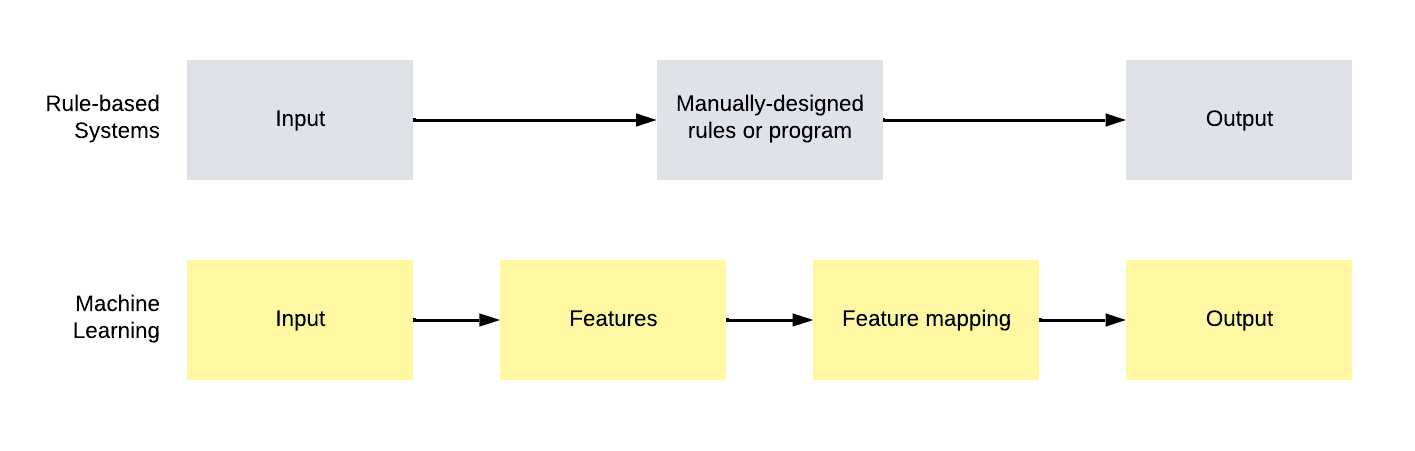
\includegraphics[width=\textwidth]{gambar/tipus_gambar_machine learning1}
	
	% Ubah dengan keterangan gambar yang diinginkan
	\caption{Perbandingan \emph{Machine Learning} dengan pemrograman biasa}
	\label{fig:machinelearning}
\end{figure}

\emph{Machine Learning} berbeda dengan pemrograman sistem tradisional yang berbasis peraturan. Seperti yang tertera pada Gambar 2.1, pemrograman tradisional memerlukan serangkaian peraturan atau program yang ditulis secara manual agar mendapatkan output yang diharapkan berdasarkan pada input yang dimasukkan. Sedangkan, pada \emph{machine learning}, tidak diperlukan untuk membuat program atau peraturannya secara manual, tapi bisa hanya dengan menentukan fitur-fitur data apa saja yang digunakan beserta hasil yang diinginkan. Secara otomatis, sistem akan mengoutputkan sebuah prediksi yang berdasarkan pada analisis dari data fitur dan algoritma statistika.

\subsection{Supervised Learning}
\label{sec:supervisedlearning}
Pada Supervised Learning, sistem akan menerima sejumlah contoh data yang telah dilabel untuk melakukan training dan membuat prediksi terhadap poin-poin yang belum terlihat. Metode ini paling sering ditemui pada permasalahan klasifikasi, regresi, dan ranking \citep{mohri2012foundations}. Supervised Learning dapat mengetahui suatu skenario dimana pada suatu contoh data training memiliki informasi signifikan yang tidak ada pada contoh data yang belum pernah dilihat. Dengan ini, maka diharapkan sistem dapat memprediksikan informasi yang tidak ada pada test data. Sistem ini dapat dianalogikan seperti seorang guru yang menjadi seorang supervisor terhadap muridnya dengan cara memberikan informasi tambahan, yaitu berupa label \citep{shalev2014understanding}.

\subsection{Unsupervised Learning}
\label{sec:unsupervisedlearning}
Pada Unsupervised Learning, sistem akan menerima sejumlah data tanpa label untuk melakukan training dan membuat prediksi terhadap poin-poin yang belum terlihat. Dikarenakan pada umumnya tidak ada contoh yang berlabel pada skenario tersebut maka akan lebih sulit untuk mengevaluasikan performa dari sistem secara kuantitatif. Contoh dari permasalahan Unsupervised Learning adalah seperti clustering dan dimensionality reduction \citep{mohri2012foundations}. Tidak ada perbedaan antara training dan test data pada unsupervised learning. SIstem akan memproses data input dengan tujuan untuk dapat mengambil suatu kesimpulan atau membuat kompresi dari data tersebut \citep{shalev2014understanding}.

\section{Deep Learning}
\label{sec:deeplearning}

Pada Gambar 2.2 tertera bahwa \emph{machine learning} merupakan suatu teknologi yang masih menjadi cakupan dari \emph{Artificial Intelligence} (AI). \emph{Deep learning} sendiri merupakan contoh dari \emph{representation learning}. Begitu pula dengan \emph{representation learning} merupakan contoh dari \emph{machine learning}. Teknologi seperti \emph{machine learning} dan \emph{representation learning} dinilai masih kurang mampu dalam menganalisis suatu data yang lebih kompleks dan memiliki sifat yang abstrak.

\begin{figure}[H]
	\centering
	
	% Ubah dengan nama file gambar dan ukuran yang akan digunakan
	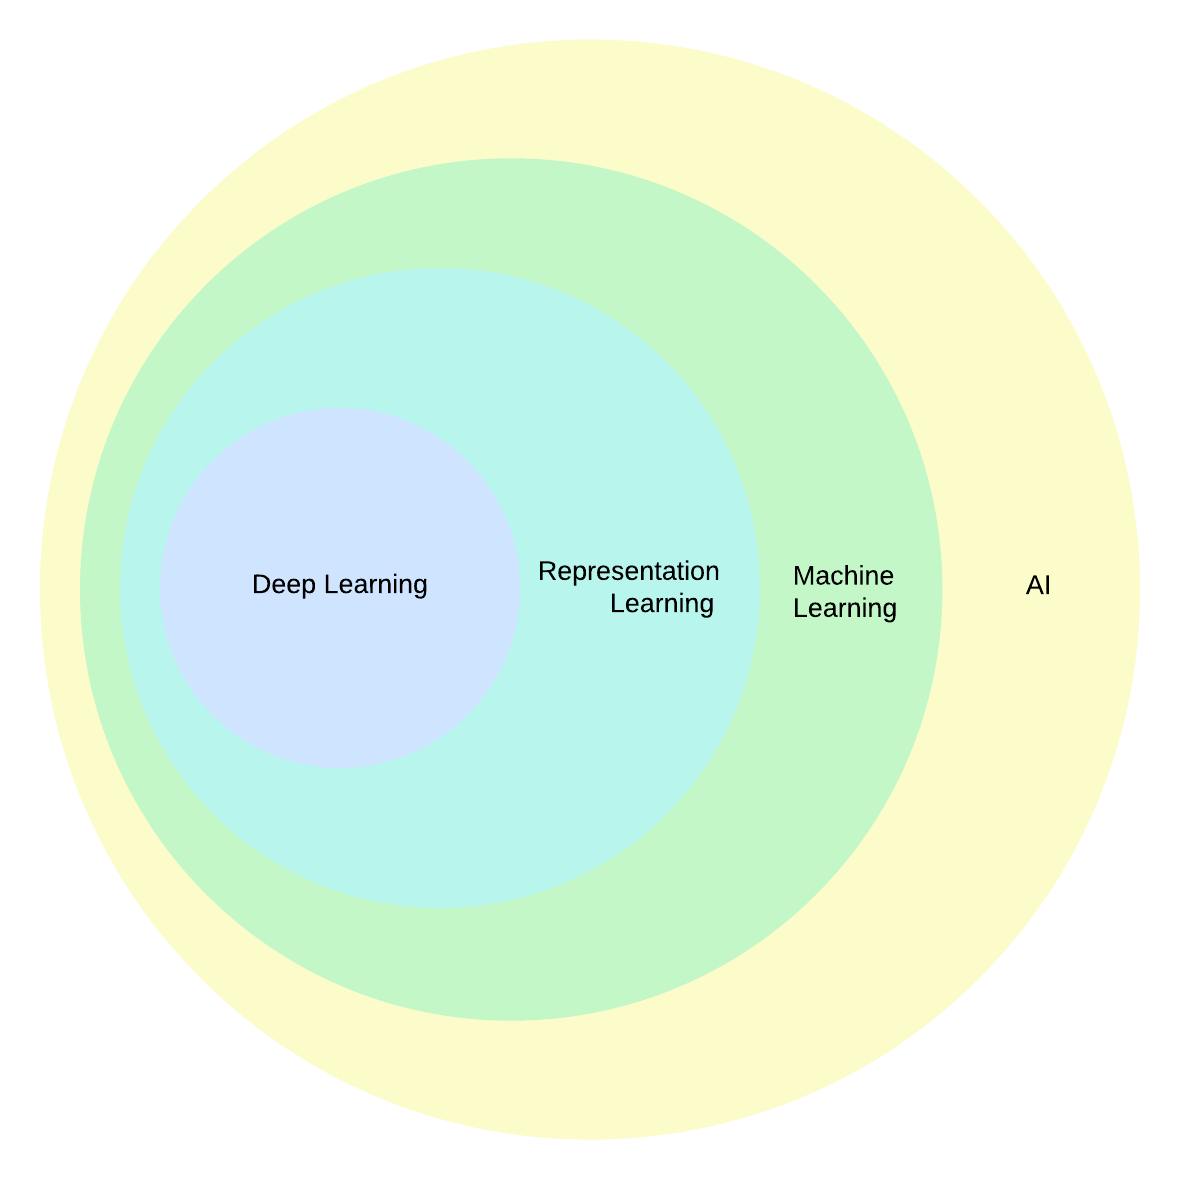
\includegraphics[width=0.8\textwidth]{gambar/tipus_gambar_deep learning venn}
	
	% Ubah dengan keterangan gambar yang diinginkan
	\caption{Diagram Venn teknologi \emph{Artificial Intelligence} (AI)}
	\label{fig:deeplearningvenn}
\end{figure}

Pada dunia pengaplikasian \emph{artificial intelligence} kesulitan yang sering dihadapi disebabkan oleh banyaknya variasi faktor-faktor yang mempengaruhi data yang sedang diobservasi. Sebagai contoh, tiap-tiap piksel dari sebuah gambar mobil berwarna merah akan lebih mendekati warna hitam pada malam hari. Selain itu, bentuk dari siluet mobil juga akan berubah-ubah bergantung pada sudut pandangnya. Umumnya, faktor-faktor variasi semacam ini perlu untuk diuraikan dan untuk variasi lain yang tidak diperlukan dapat diabaikan saja.

Tentunya, tidaklah mudah untuk mengekstrak fitur-fitur yang abstrak seperti yang disebutkan tadi melalui data mentahan. Contoh lainnya adalah seperti aksen dari seorang pembicara yang hanya dapat diidentifikasikan melalui kecerdasan yang mendekati kemampuan manusia dalam memahami hal tersebut. Deep Learning dapat menyeleaikan permasalahan seperti ini karena komputer dapat membangun suatu konsep yang kompleks dari hal yang sederhana. Salah satu contoh paling penting dari model \emph{deep learning} adalah seperti \emph{feed forward deep neutwork} atau \emph{multilayer perceptron} (MLP). \emph{Multilayer perceptron} adalah sebuah fungsi matematika yang memetakan nilai-nilai input ke output. Fungsi ini dibentuk dengan cara menggabungkan fungsi-fungsi yang lebih sederhana dan setiap fungsi ini akan memengaruhi hasil representasi dari input \citep{deepL}.

\begin{figure}[H]
	\centering
	
	% Ubah dengan nama file gambar dan ukuran yang akan digunakan
	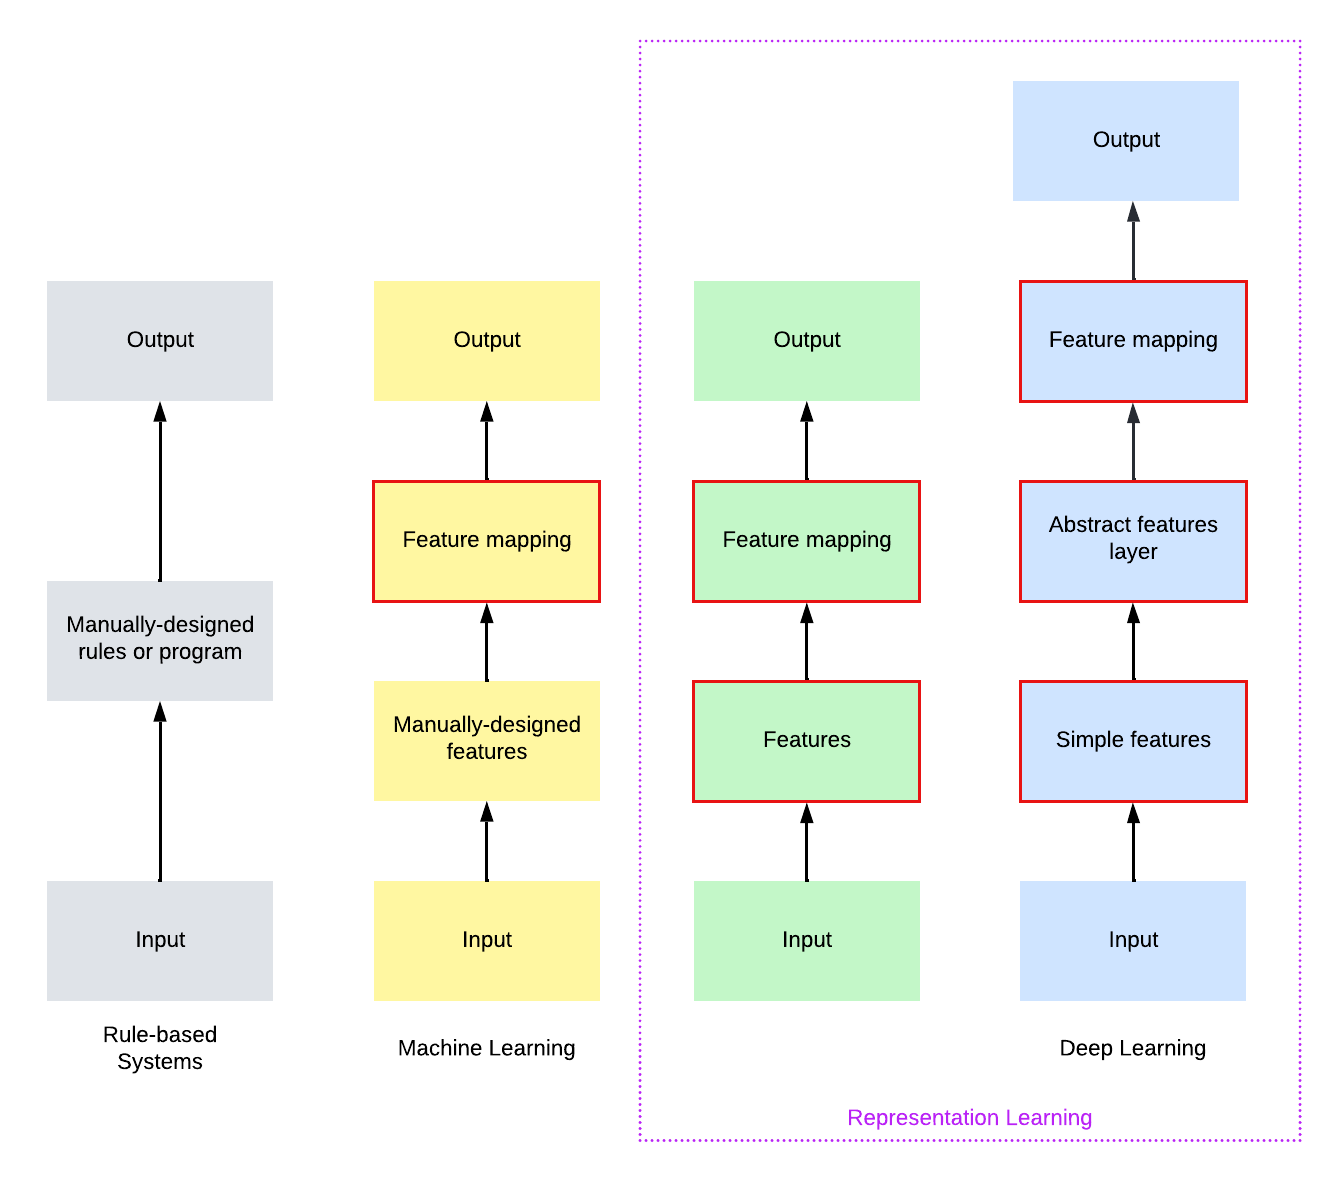
\includegraphics[width=0.8\textwidth]{gambar/tipus_gambar_deep learning}
	
	% Ubah dengan keterangan gambar yang diinginkan
	\caption{Perbandingan masing-masing teknologi \emph{machine learning} dan pemrograman biasa}
	\label{fig:deeplearningdiagram}
\end{figure}

Seperti yang telah dipaparkan pada Subbab 2.5 terlihat perbedaan dari \emph{machine learning} dengan pemrograman tradisional. Namun, masing-masing teknologi dari \emph{machine learning} sendiri memiliki beberapa perbedaan pula. Pada \emph{machine learning} klasik diperlukan fitur-fitur data yang didesain secara manual yang kemudian akan dilakukan pemetaan fitur. Kotak yang diberi \emph{outline} berwarna merah melambangkan bahwa komponen tersebut dapat dilakukan secara otomatis (dipelajari) oleh sistem. Berbeda dengan dengan \emph{representation learning} yang di mana sistem dapat memilih fitur-fitur yang diperlukan secara otomatis. Pada \emph{deep learning}, dibandingkan dengan \emph{representation learning}, hanya memerlukan fitur-fitur data simpel yang kemudian akan ditambahkan beberapa layer tambahan berisikan fitur-fitur yang lebih abstrak.

%Deep Learning merupakan salah satu pendekatan kecerdasan buatan dan tipe dari pembelajaran mesin. Deep Learning adalah salah satu jenis pembelajaran mesin yang dapat mencapai kekuatan yang tinggi serta fleksibilitas belajar untuk merepresentasikan dunia sebagai sebuah konsep nested hierarchy yang tiap-tiap konsepnya didefinisikan dalam kaitannya dengan konsep yang lebih sederhana, serta representasi yang lebih abstrak dikomputasikan dengan cara yang lebih tidak abstrak \citep{deepL}.

% input gambar
%\begin{figure} [H] \centering
% Nama dari file gambar yang diinputkan
%\includegraphics[scale=0.6]{gambar/umur.png}
% Keterangan gambar yang diinputkan
%\caption{Kategori umur menurut Depkes. RI (2009)}
% Label referensi dari gambar yang diinputkan
% \label{fig:Umur}
%\end{figure}

\section{Convolutional Neural Network (CNN)}
\label{sec:cnn}
Convolutional Neural Network adalah salah satu jenis dari neural network untuk memproses data yang memiliki topologi seperti grid. Contohnya adalah, data time-series yang dimana dapat digambarkan sebagai sebuah grid 1 dimensi yang mengambil sampel pada suatu interval waktu, dan data gambar yang dimana dapat dikatakan sebagai sebuah grid 2 dimensi berisikan piksel-piksel. Nama dari “Convolutional Neural Network” itu sendiri mengimplikasikan bahwa suatu network menggunakan operasi matematika yang disebut sebagai konvolusi. Konvolusi sendiri merupakan salah satu jenis dari operasi linear. Convolutional Network adalah sebuah neural network yang menggunakan konvolusi sebagai pengganti matriks perkalian umum di minimal salah satu lapisannya \citep{deepL}.

\section{\emph{Music Information Retrieval} (MIR)}
\label{sec:mir}

Music Information Retrieval (MIR) pertama diperkenalkan oleh Michael Kassler pada pertengahan dekade 1960-an. Perkembangan signifikan dari MIR ini diikuti oleh pertama kali didirikannya International Symposium on Music Information Retrieval (ISMIR) pada tahun 2000. Tujuan utama dari MIR adalah untuk memperbaiki akses penggemar musik terhadap koleksi musik dengan jumlah yang besar \citep{lefaivre2019characterizing}, terutama dengan berkembangnya platform-platform musik digital daring, jumlah pengguna maupun jumlah musik yang masuk ke dalam database juga makin besar sehingga diperlukan suatu sistem untuk mempermudah akses pengguna terhadap database musik tersebut. 

Penyimpanan dari musik sendiri dapat dibedakan menjadi dua kategori yang paling populer, yaitu continuous atau raw. Contoh dari formatnya adalah seperti MP3, wav, atau AIFF yang dimana juga menggambarkan kualitas dari audionya. Biasanya file-file tersebut disimpan dengan kualitas dan sample rate yang bermacam-macam. Contoh lain yang lebih jarang ditemui adalah pada format discrete, yaitu seperti MIDI, atau GUIDO. Format seperti ini biasanya secara digital dapat menggambarkan niatan dari si komposer meskipun biasanya format continuous memiliki jumlah data dan informasi yang jauh lebih banyak. Konversi antara kedua format biasanya hanya dapat dilakukan searah, yaitu dari discrete ke continuous \citep{McDermott2005TheSO}. 

\section{\emph{Mel-Frequency Coefficient of Cepstrum} (MFCC)}
\label{sec:mfcc}
%Mel-Frequency Cepstrum sangat efektif digunakan pada pengenalan suara, serta pemodelan subjective pitch dan konten frekuensi pada sinyal audio \citep{hmmaudio}.

Mel-Frequency Ceptral Coefficient (MFCC), dikembangkan oleh Davis dan Memelstein, merupakan sebuah metode ekstraksi fitur audio dengan cara menghitung koefisien ceptral berdasarkan variasi frekuensi kritis pada pendengaran manusia \citep{Widodo2017PenerapanMM}.
MFCC merepresentasikan sinyal pelafalan menjadi bentuk parametris untuk mempermudah pemrosesan dan analisis. Skala pitch yang memiliki jarak yang sama satu dengan lainnya disebut sebagai mel scale \citep{audiosignal1}.
MFCC merupakan fitur audio berbasis cepstrum yang paling sering digunakan. Hal ini dikarenakan MFCC dapat merepresentasikan vektor fitur dari sinyal musik maupun pelafalan, selain itu juga terbukti sangat berguna untuk klasifikasi audio pada umumnya \citep{li2019digital}.

\section{\emph{Confusion Matrix}}
\label{sec:confmatrix}

Confusion matrix adalah sebuah tabel yang merepresentasikan performa dari suatu model klasifikasi dalam memprediksi data ke berbagai macam class. Apabila sumbu x melambangkan prediction label maka sumbu y melambangkan true label-nya. Salah satu contohnya ada pada klasifikasi biner yang dimana hanya terdapat 2 class. Berikut seperti yang tertera pada Tabel 2.1 contoh dari tabel \emph{confusion matrix} untuk klasifikasi biner antara teks \emph{Spam} dan \emph{Not Spam}.

\begin{longtable}[c]{|c|c|c|}
	\caption{Contoh sederhana \emph{confusion matrix}}
	\label{tab:my-table}\\
	\hline
	& \textbf{Spam (predicted label)} & \textbf{Not Spam (predicted label)} \\ \hline
	\endfirsthead
	%
	\endhead
	%
	\textbf{Spam (true label)}     & 43 (TP)                         & 7 (FN)                              \\ \hline
	\textbf{Not Spam (true label)} & 11 (FP)                         & 39 (TN)                             \\ \hline
\end{longtable}

Seperti yang terlihat pada Tabel 2.1, terdapat 2 sumbu, yaitu kolom \emph{predicted label} dan baris \emph{true label}. \emph{True label} melambangkan label asli dari data, sedangkan \emph{predicted label} melambangkan label yang terprediksi oleh sistem. Dapat dilihat terdapat 43 data yang terprediksi dengan benar oleh sistem sebagai sebuah teks \emph{Spam}. Hal ini disebut sebagai \emph{True Positive} (TP). Selanjutnya terdapat pula data yang terprediksi sebagai sebuah \emph{Spam}, namun sebenarnya adalah \emph{Not Spam}, yaitu sebanyak 11 data. Hal ini disebut sebagai \emph{False Positive} (FP). Sebaliknya, juga terdapat data teks yang sebenarnya \emph{Not Spam} dan terprediksi oleh sistem dengan benar, yaitu sebanyak 39 data. Hal ini disebut sebagai \emph{True Negative} (TN). Terakhir, terdapat data yang terprediksi sebagai \emph{Not Spam} walaupun sebenarnya merupakan data teks \emph{Spam}, yaitu sebanyak 7 data. Hal ini disebut sebagai \emph{False Negative} (FN).